\chapter{lectureEditor}

\section{Grundlagen des Arbeitsbereichs}

\begin{figure}[H]
	\centering
	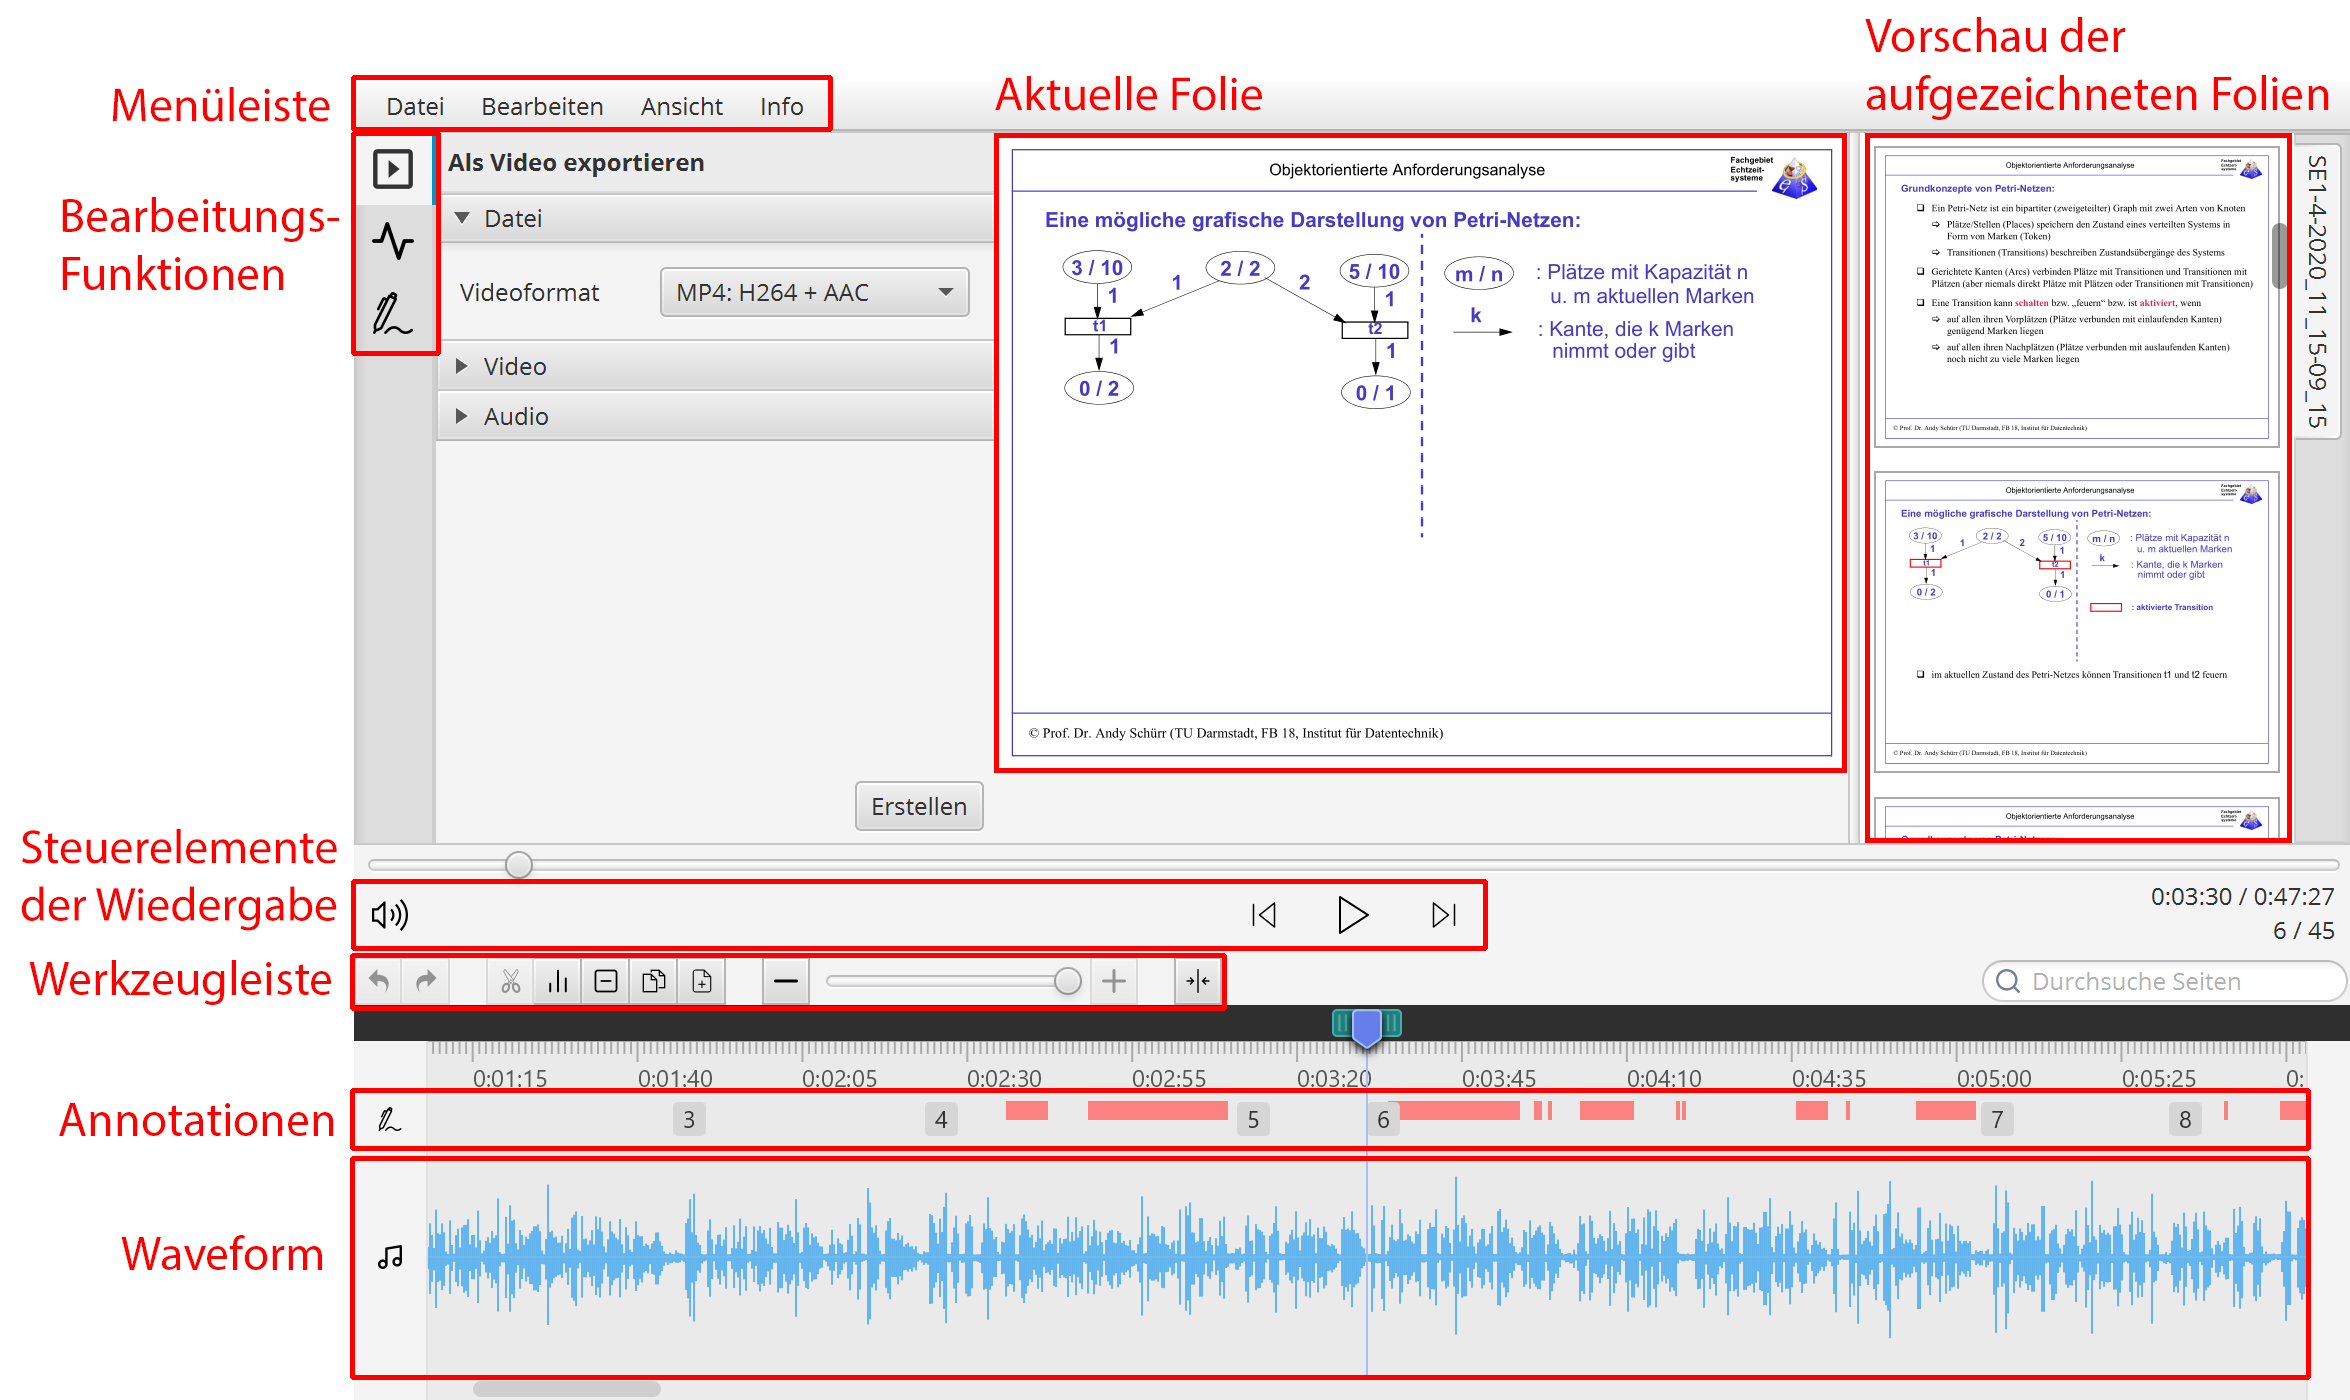
\includegraphics[width=0.95\textwidth]{editor/editor-main}
	\caption{\lectEditor}
	\label{fig:\lectEditor}
\end{figure}

\subsection{Werkzeuge}
\label{section:editor:toolbar}

\begin{figure}[H]
	\centering
	
\includegraphics[width=0.7\linewidth]{editor/editor-toolbar}
	\caption{\lectEditor{}-Werkzeugleiste}
	\label{fig:editor-toolbar}
\end{figure}


\begin{longtable}{p{1cm}p{12cm}}
	\begin{minipage}{.035\textwidth}
		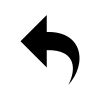
\includegraphics[width=\linewidth]{editor/editor-undo}
	\end{minipage}
	& Letzten Bearbeitungsschritt rückgängig machen. \\

	\begin{minipage}{.035\textwidth}
		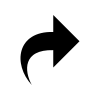
\includegraphics[width=\linewidth]{editor/editor-redo}
	\end{minipage}
	& Gelöschten Bearbeitungsschritt wiederherstellen. \\

	\begin{minipage}{.035\textwidth}
		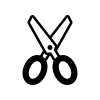
\includegraphics[width=\linewidth]{editor/editor-cut}
	\end{minipage}
	& Aktuellen Auswahlbereich entfernen. \\

	\begin{minipage}{.035\textwidth}
		
\includegraphics[width=\linewidth]{editor/adjust-volume}
	\end{minipage}
	& Lautstärke im Auswahlbereich anpassen. \\

	\begin{minipage}{.035\textwidth}
		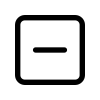
\includegraphics[width=\linewidth]{editor/editor-cut-page}
	\end{minipage}
	& Aktuelle Folie entfernen. \\

	\begin{minipage}{.035\textwidth}
		
\includegraphics[width=\linewidth]{editor/replace-page}
	\end{minipage}
	& Aktuelle Folie durch eine andere ersetzen. \\

	\begin{minipage}{.035\textwidth}
		
\includegraphics[width=\linewidth]{editor/editor-import}
	\end{minipage}
	& Eine Aufzeichnung an die aktuelle Zeitmarker-Position importieren. \\

	\begin{minipage}{.035\textwidth}
		
\includegraphics[width=\linewidth]{editor/editor-zoom-in}
	\end{minipage}
	& In die Waveform reinzoomen. \\

	\begin{minipage}{.035\textwidth}
		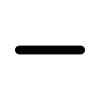
\includegraphics[width=\linewidth]{editor/editor-zoom-out}
	\end{minipage}
	& Aus der Waveform rauszoomen. \\

	\begin{minipage}{.035\textwidth}
		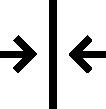
\includegraphics[width=\linewidth]{editor/collapse-selection}
	\end{minipage}
	& Auswahlbereich zusammenführen. \\
\end{longtable}

\section{Anwendungsszenarien}
In diesem Kapitel werden häufige Anwendungsszenarien sowie deren Nutzung in \lectEditor{} beschrieben.

\subsection{Schneiden}
Um Stille, einen Fehler oder einen unnötigen Abschnitt aus der Aufnahme zu löschen, markieren Sie diesen Bereich in der Waveform mit den Zeitmarkern.

\newcommand{\editorslider}{%
  \begingroup\normalfont
  
\includegraphics[height=\fontcharht\font`\B]{editor/slider}%
  \endgroup
}
\newcommand{\editorsecondarysliderleft}{%
  \begingroup\normalfont
  
\includegraphics[height=\fontcharht\font`\B]{editor/slider-left}%
  \endgroup
}
\newcommand{\editorsecondarysliderright}{%
  \begingroup\normalfont
  
\includegraphics[height=\fontcharht\font`\B]{editor/slider-right}%
  \endgroup
}
\newcommand{\editorundo}{%
  \begingroup\normalfont
  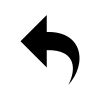
\includegraphics[height=\fontcharht\font`\B]{editor/editor-undo}%
  \endgroup
}
\newcommand{\editorcut}{%
  \begingroup\normalfont
  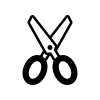
\includegraphics[height=\fontcharht\font`\B]{editor/editor-cut}%
  \endgroup
}
\newcommand{\editoradjustvolume}{%
  \begingroup\normalfont
  
\includegraphics[height=\fontcharht\font`\B]{editor/adjust-volume}%
  \endgroup
}
\newcommand{\editorcollapseselection}{%
  \begingroup\normalfont
  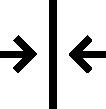
\includegraphics[height=\fontcharht\font`\B]{editor/collapse-selection}%
  \endgroup
}
\newcommand{\editorcutpage}{%
  \begingroup\normalfont
  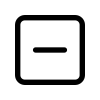
\includegraphics[height=\fontcharht\font`\B]{editor/editor-cut-page}%
  \endgroup
}
\newcommand{\editorreplacepage}{%
  \begingroup\normalfont
  
\includegraphics[height=\fontcharht\font`\B]{editor/replace-page}%
  \endgroup
}
\newcommand{\editorplay}{%
  \begingroup\normalfont
  
\includegraphics[height=\fontcharht\font`\B]{editor/editor-play}%
  \endgroup
}

\begin{enumerate}
	\item Navigieren Sie in der Waveform an die gewünschte Position.
	\item Bewegen Sie den Zeitmarker \editorslider{} oder die sekundären Zeitmarker \editorsecondarysliderleft{}\editorsecondarysliderright{} nach links oder rechts, um den gewünschten Bereich auszuwählen.

	Der ausgewählte Bereich ist vom grünen Rechteck umschlossen (\autoref{fig:timeline-select}).

	\begin{minipage}{0.9\textwidth}
		\centering
		\captionsetup{type=figure}
		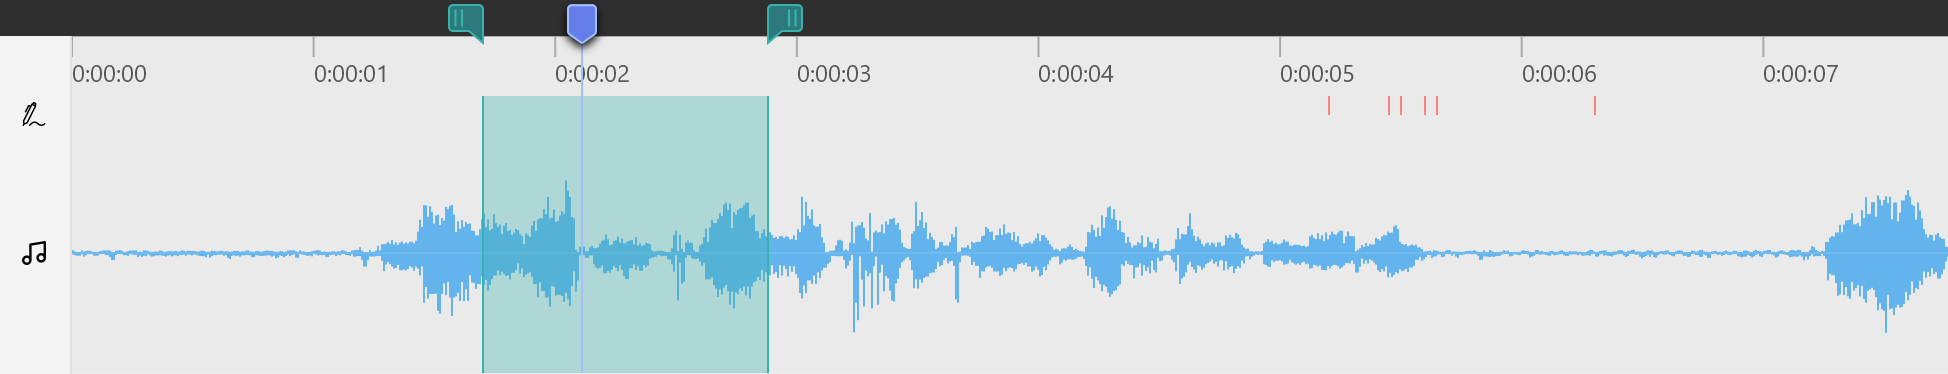
\includegraphics[width=0.9\textwidth]{editor/timeline-select}
		\captionof{figure}{Auswahlbereich}
		\label{fig:timeline-select}
	\end{minipage}

	\item Klicken Sie auf \quote{Ausschneiden} \editorcut{} über der Waveform.
	
	Dadurch wird der Auswahlbereich entfernt. Alle darauffolgenden Folien samt Annotationen werden nach links verschoben, um die Lücke zu schließen.
\end{enumerate}

\subsubsection{Komplette Folie entfernen}
Folien samt Annotationen lassen sich auch ohne die Auswahl mit Zeitmarkern in der Waveform entfernen.

\begin{enumerate}
	\item Navigieren Sie auf eine Folie, die Sie komplett entfernen möchten.
	\item Klicken Sie auf \quote{Aktuelle Seite entfernen} \editorcutpage{} über der Waveform.
\end{enumerate}

\textbf{Alternativ:}

\begin{enumerate}
	\item Rechtsklick mit der Maus auf die Folie in der Vorschauleiste (\autoref{fig:editor-delete-page}).
	
	\begin{minipage}{0.9\textwidth}
		\centering
		\captionsetup{type=figure}
		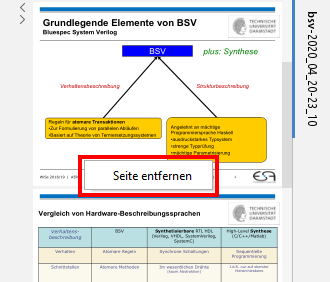
\includegraphics[width=0.5\textwidth]{editor/editor-delete-page}
		\captionof{figure}{Komplette Folie aus der Aufzeichnung entfernen}
		\label{fig:editor-delete-page}
	\end{minipage}

	\item Klicken Sie auf \quote{Seite entfernen} im Kontextmenü.
\end{enumerate}


\subsection{Folie ersetzen}
Sie können Folien im aufgezeichneten Dokument ersetzen. Diese Funktion ist hilfreich, wenn Sie eine Aufzeichnung wiederverwenden und zum Beispiel nur das Datum anpassen möchten, oder Fehler wie beispielsweise Rechtschreibfehler beheben möchten. Alle Annotationen, die auf dieser Folie gemacht wurden bleiben unverändert erhalten.

\begin{enumerate}
	\item Navigieren Sie auf eine Folie, die Sie ersetzen möchten.
	\item Klicken Sie auf \quote{Aktuelle Seite ersetzen} \editorreplacepage{} über der Waveform.
	\item Im Datei-Auswahl-Dialog einen Foliensatz auswählen, in dem sich die neue Folie befindet.
	\item Wählen Sie im Foliensatz die neue Folie aus und klicken \keys{Ersetzen}.
	\item Die ausgewählte Folie wurde ersetzt.
\end{enumerate}


\subsection{Lautstärke anpassen}
Es kann vorkommen, dass Sie die Lautstärke in einzelnen Passagen ihrer Aufzeichnung verändern möchten. Dies kann zum Beispiel nach dem Einfügen einer neuen Passage der Fall sein.

\begin{enumerate}
	\item Navigieren Sie in der Waveform an die gewünschte Position.
	\item Bewegen Sie den Zeitmarker \editorslider{} oder die sekundären Zeitmarker \editorsecondarysliderleft{}\editorsecondarysliderright{} nach links oder rechts, um den gewünschten Bereich auszuwählen.

	Der ausgewählte Bereich ist vom grünen Rechteck umschlossen (\autoref{fig:timeline-select-2}).

	\begin{minipage}{0.9\textwidth}
		\centering
		\captionsetup{type=figure}
		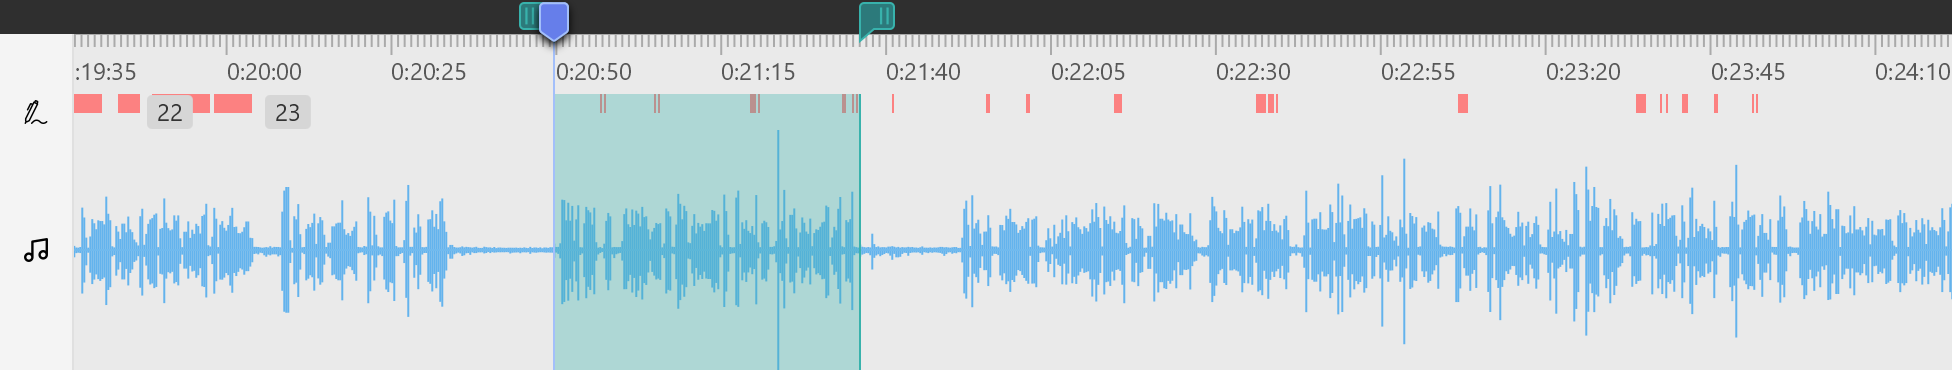
\includegraphics[width=0.9\textwidth]{editor/timeline-select-2}
		\captionof{figure}{Auswahlbereich zur Anpassung der Lautstärke}
		\label{fig:timeline-select-2}
	\end{minipage}

	\item Klicken Sie auf \quote{Lautstärke anpassen} \editoradjustvolume{} über der Waveform. Es wird ein neuer violetter Auswahlbereich für die Anpassung der Lautstärke erstellt.
	
	\item Im violetten Auswahlbereich können Sie nun die Lautstärke anpassen (\autoref{fig:timeline-adjust-volume}). Bewegen Sie den horizontalen Balken nach oben, um die Lautstärke zu erhöhen, oder nach unten, um sie zu senken [1]. Die Änderung ist sofort in der Waveform sichtbar.

	\begin{minipage}{0.9\textwidth}
		\centering
		\captionsetup{type=figure}
		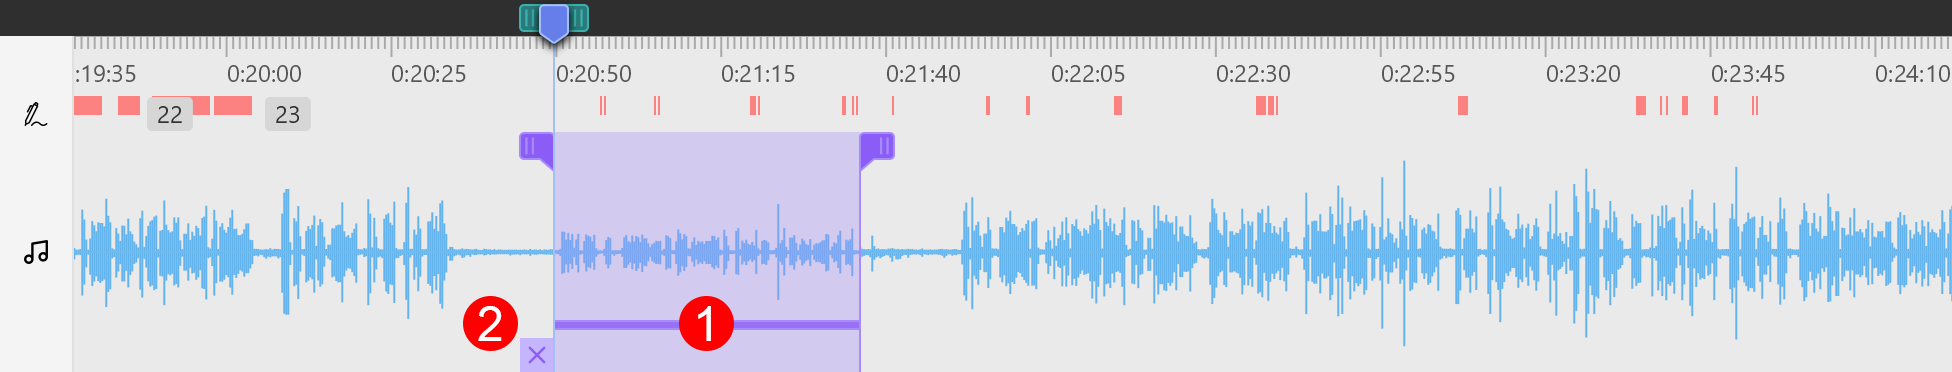
\includegraphics[width=0.9\textwidth]{editor/timeline-adjust-volume}
		\captionof{figure}{Lautstärke anpassen im Auswahlbereich}
		\label{fig:timeline-adjust-volume}
	\end{minipage}

	\begin{note}
		Es wird empfohlen den grünen Auswahlbereich mit \editorcollapseselection{} zusammenzufalten.
	\end{note}

	\item Sollten Sie es sich anders überlegt haben, so können Sie die Anpassung mit \keys{X} [2] oder \editorundo{} entfernen.
\end{enumerate}


\subsection{Rauschunterdrückung}
Je nach Qualität des Mikrofons, wird neben der Sprache auch Rauschen aufgezeichnet. Um die Sprachverständlichkeit zu erhöhen kann ein Rauschunterdrückungsverfahren angewandt werden. Da statistische Rauschsignale sich im Allgemeinen nicht gut komprimieren lassen, führt die Rauschunterdrückung zu einer Reduktion der Dateigröße einer komprimierten Video-Aufzeichnung.

\begin{enumerate}
	\item Wählen Sie in der Waveform mit den Zeitmarkern einen Bereich mit Stille aus, d.h. ohne Sprach-/Audiosignal. Die Pegel sind in der Waveform nahe der Mittellinie (\autoref{fig:timeline-silence}).
	
	\begin{minipage}{0.9\textwidth}
		\centering
		\captionsetup{type=figure}
		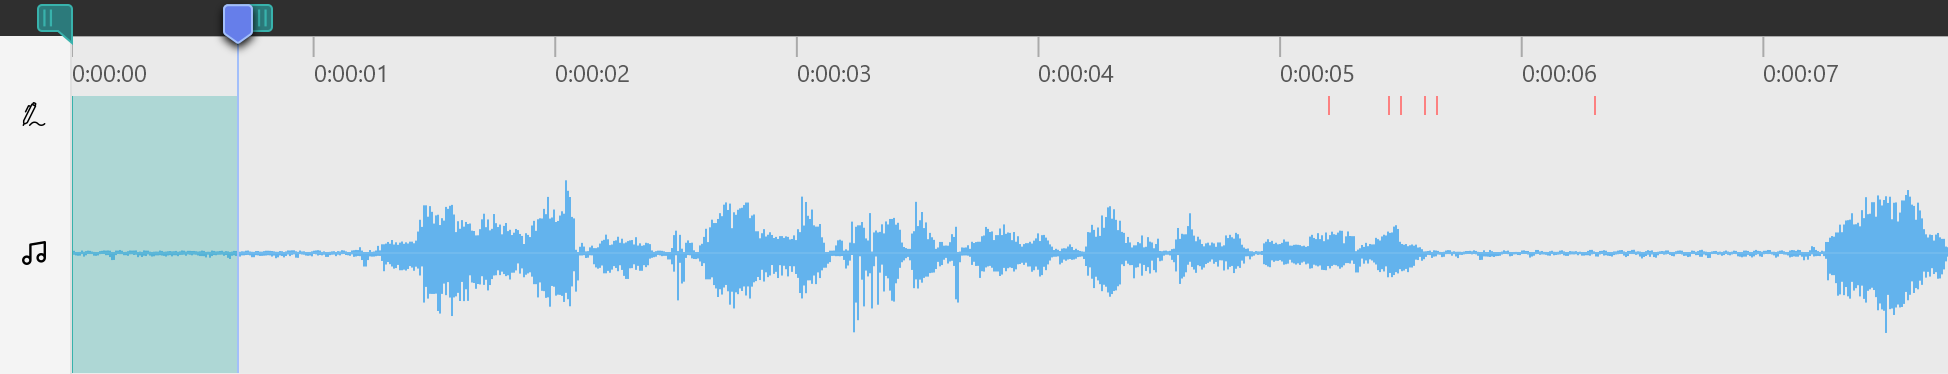
\includegraphics[width=0.9\textwidth]{editor/timeline-silence}
		\captionof{figure}{Stille auswählen}
		\label{fig:timeline-silence}
	\end{minipage}

	\item Über Menü \menu[,]{Effekt, Markiertes Zeitintervall als Stille definieren} wird das Rauschsignal analysiert.
	\item Über Menü \menu[,]{Effekt, Entrauschen} öffnen Sie den Dialog zur Rauschunterdrückung (\autoref{fig:editor-nr-dialog}).

	\begin{minipage}{0.9\textwidth}
		\centering
		\captionsetup{type=figure}
		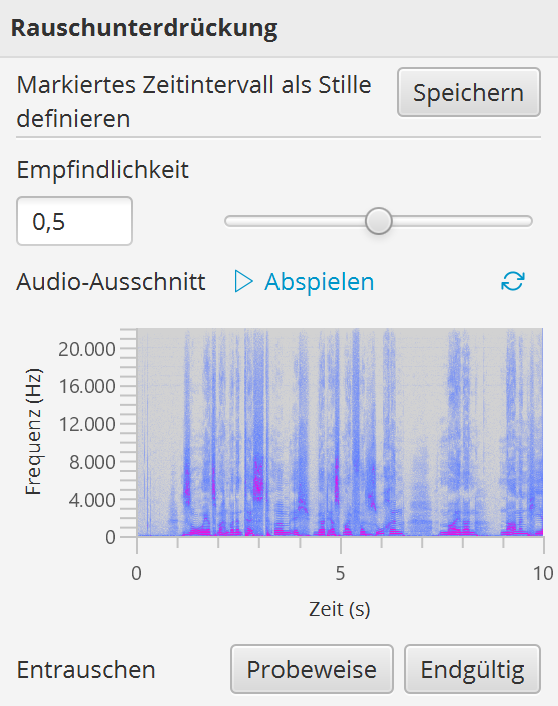
\includegraphics[width=0.5\textwidth]{editor/editor-nr-dialog}
		\captionof{figure}{Rauschunterdrückung}
		\label{fig:editor-nr-dialog}
	\end{minipage}

	\item Der Standardwert der Empfindlichkeit ist so eingestellt, dass er für die meisten Aufzeichnungen nicht verändert werden muss. Um sicher zu gehen, ob die Empfindlichkeit der Rauschunterdrückung passt, führen Sie den nächsten Schritt aus.
	
	\begin{info}
		Je höher der Wert, desto mehr Signale werden aus der Aufzeichnung entfernt. Ein zu hoher Wert beeinträchtigt die Qualität der Sprache, da auch hier die dazugehörenden Frequenzen unterdrückt werden.
	\end{info}

	\item Sie können probeweise entrauschen und vorhören. Dazu klicken Sie zunächst \keys{Probeweise entrauschen} und dann \editorplay{}.
	
	Eine Veränderung des Spektrogramms ist in \autoref{fig:editor-nr-dialog-test} zu sehen. Es ist zu erkennen, dass hauptsächlich Frequenzen der Sprache übrig geblieben sind.
	
	Wenn Sie mit dem Resultat nicht zufrieden sind, dann verstellen Sie die Empfindlichkeit und klicken erneut \keys{Probeweise entrauschen}.

	\begin{minipage}{0.9\textwidth}
		\centering
		\captionsetup{type=figure}
		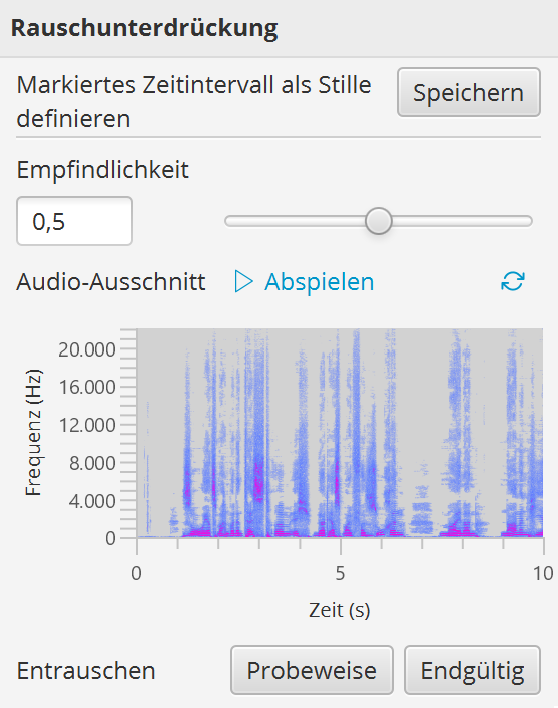
\includegraphics[width=0.5\textwidth]{editor/editor-nr-dialog-test}
		\captionof{figure}{Probeweise Rauschunterdrückung}
		\label{fig:editor-nr-dialog-test}
	\end{minipage}

	\item Damit die Rauschunterdrückung auf die gesamte Aufzeichnung angewandt wird, drücken Sie \keys{Endgültig entrauschen}.
	
	Der Dialog schließt sich automatisch, nachdem die Rauschunterdrückung erfolgreich durchgelaufen ist.
\end{enumerate}


\subsection{Video-Export}
Exportieren Sie Ihre Aufzeichnung als komprimiertes Video, das in allen gängigen Videoplayern wiedergegeben werden kann.

\label{section:video-export}
\begin{enumerate}
	\item Klicken Sie auf \keys{Video Erstellen} im Schnellzugriff für den Video-Export. Es öffnet sich ein Dialog (\autoref{fig:editor-video-export}).
	
	\begin{minipage}{0.9\textwidth}
		\centering
		\captionsetup{type=figure}
		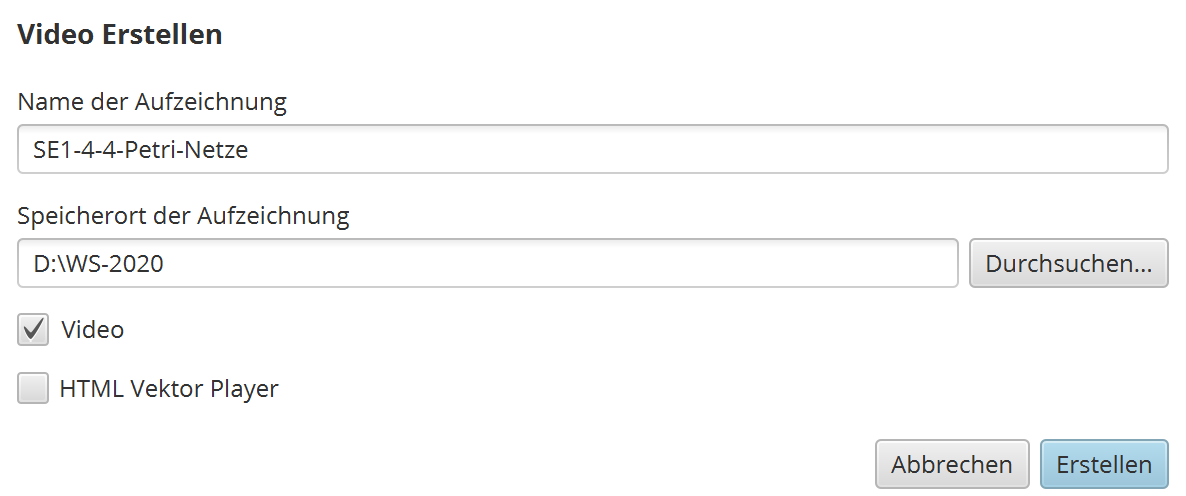
\includegraphics[width=0.65\textwidth]{editor/editor-video-export}
		\captionof{figure}{Video-Export}
		\label{fig:editor-video-export}
	\end{minipage}

	\item Wählen Sie den Speicherort aus.
	\item Aktivieren Sie die Option \quote{HTML video player}, wenn zu dem Video eine HTML-Datei mit erweiterten Funktionen wie die Textsuche und Anspringen von Folien im Video erstellt werden soll.
	
	\begin{note}
		Die HTML-Datei kann mit dem Video auf den Helios Medienserver der TU Darmstadt geladen und freigegeben werden.
	\end{note}

	Die HTML-Darstellung einer beispielhaften Aufzeichnung ist in \autoref{fig:editor-html-export} zu sehen.

	\begin{minipage}{0.9\textwidth}
		\centering
		\captionsetup{type=figure}
		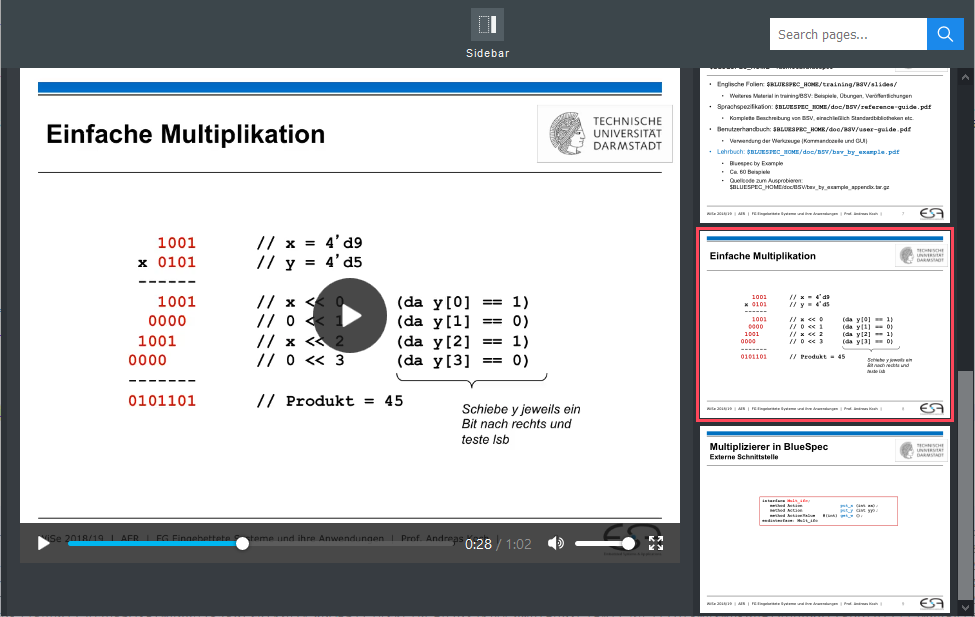
\includegraphics[width=0.7\textwidth]{editor/editor-html-export}
		\captionof{figure}{HTML Video-Export}
		\label{fig:editor-html-export}
	\end{minipage}

	\item Aktivieren Sie die Option \quote{HTML vector player}, wenn zu dem Video eine komprimierte Aufzeichnung im Vektorformat erstellt werden soll. Die damit erzeugte Aufzeichnungsdatei kann über die mitgelieferte HTML-Datei wiedergegeben werden.

	\begin{note}
		In der Regel haben komprimierte Vektor-Aufzeichnungen eine geringere Dateigröße als komprimierte Videos, haben aber den Nachteil, dass sie nur mit der HTML-Datei, die die Wiedergabe-Funktionalität implementiert, wiedergegeben werden können.
	\end{note}

	\item Klicken Sie auf \keys{Erstellen}.
	\begin{info}
		Wenn Sie die Option \quote{HTML video player} aktiviert haben, dann finden Sie im Speicherort ein Verzeichnis mit dem Namen der Aufzeichnung vor.
	\end{info}
\end{enumerate}

\textbf{Alternativ mit Experteneinstellungen:}

\begin{enumerate}
	\item Um mehr Einfluss auf die Qualität des Videos zu bekommen, klicken Sie im Menü auf \menu[,]{Ansicht, Erweiterte Einstellungen}.
	
	Sie bekommen die erweiterten Bedienelemente (\autoref{fig:editor-extended-video-export}) zu sehen.
	
	\begin{minipage}{0.9\textwidth}
		\centering
		\captionsetup{type=figure}
		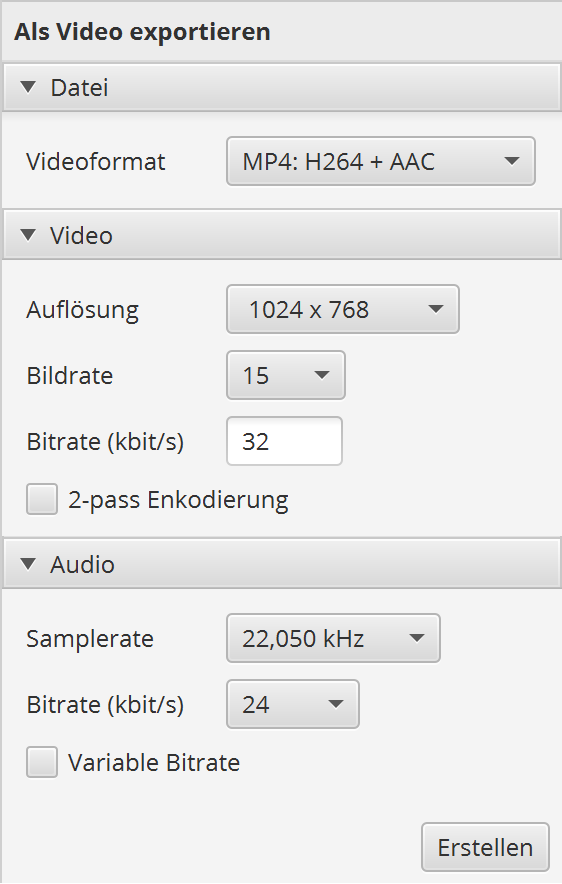
\includegraphics[width=0.5\textwidth]{editor/editor-extended-video-export}
		\captionof{figure}{Erweiterte Video-Export-Einstellungen}
		\label{fig:editor-extended-video-export}
	\end{minipage}

	\item Nehmen Sie die gewünschten Einstellungen vor. Die Standardwerte sind so eingestellt, dass ein Video mit guter Qualität und geringer Dateigröße erstellt wird.
	
	\begin{info}
		Je höher die Werte, desto besser ist die Qualität des Videos. Mit besserer Qualität erhöht sich auch die Dateigröße des Videos.
	\end{info}

	\item Anschließend klicken Sie auf \keys{Video Erstellen} und fahren mit den zuvor beschriebenen Schritten im Absatz \ref{section:video-export} fort.
\end{enumerate}

\vfill

\pagebreak
\section{Tastenbelegung}

\begin{longtable}{|p{3,5cm}|l|}
	\hline
	{\ctrlKey} + O & Aufzeichnung öffnen.\\
	\hline
	{\ctrlKey} + F4 & Aufzeichnung schließen.\\
	\hline
	{\ctrlKey} + Q & Programm beenden.\\
	\hline
	{\altKey} + Enter & Vollbildmodus umschalten.\\
	\hline
	{\ctrlKey} + Z & Letzten Bearbeitungsschritt rückgängig machen.\\
	\hline
	{\ctrlKey} + Y & Gelöschten Bearbeitungsschritt wiederherstellen.\\
	\hline
	{\ctrlKey} + X & Aktuellen Auswahlbereich entfernen.\\
	\hline
	{\ctrlKey} + D & Aktuelle Folie entfernen.\\
	\hline
	\caption{\lectEditor{}-Tastenbelegung}
	\label{tab:editor-shortcuts}
\end{longtable}